%=============================================================================
\section{Softwarové inženýrství}
%=============================================================================

\subsection{UML diagramy}

\textbf{UML (Unified Modeling Language)} je standardizovaný jazyk pro vizuální modelování softwarových systémů.
Diagramy UML se dělí do dvou skupin:

\begin{itemize}
  \item \textbf{Strukturální diagramy} -- statická struktura systému: class, object, component, deployment, package
  \item \textbf{Behaviorální diagramy} -- dynamické chování: use case, sequence, activity, state machine, communication
\end{itemize}

\subsubsection{Diagram případů užití (Use Case Diagram)}

Zobrazuje interakce mezi systémem a jeho aktéry. Odpovídá na otázku: \textit{Co systém dělá?}

\textbf{Elementy:}
\begin{itemize}
  \item \textbf{Aktér (Actor)} -- role uživatele nebo externího systému; reprezentován panáčkem
  \item \textbf{Případ užití (Use Case)} -- funkce systému z pohledu aktéra; reprezentován elipsou
  \item \textbf{Vztahy:}
    \begin{itemize}
      \item \textit{Include} ($\langle\langle$include$\rangle\rangle$) -- vždy se zahrne základní UC při provádění tohoto
      \item \textit{Extend} ($\langle\langle$extend$\rangle\rangle$) -- volitelně rozšiřuje základní UC za určitých podmínek
      \item \textit{Generalizace} -- jeden aktér/UC je specializací jiného
    \end{itemize}
  \item \textbf{Hranice systému} -- obdélník oddělující systém od aktérů
\end{itemize}

\begin{figure}[H]
\centering
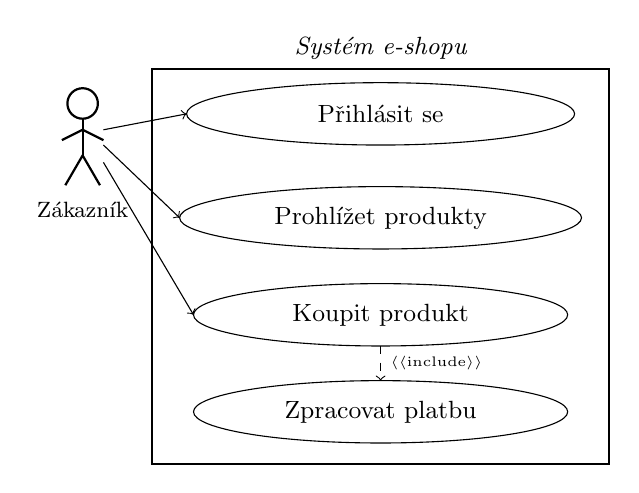
\begin{tikzpicture}[font=\small, scale=0.88]
  % System boundary
  \draw[thick] (1.0,-4.4) rectangle (7.6,1.3);
  \node[above, font=\small\itshape] at (4.3,1.3) {Systém e-shopu};
  % Stick figure actor
  \draw[thick] (0,0.8) circle (0.22);
  \draw[thick] (0,0.58) -- (0,0.05);
  \draw[thick] (-0.30,0.27) -- (0,0.42) -- (0.30,0.27);
  \draw[thick] (-0.25,-0.38) -- (0,0.05) -- (0.25,-0.38);
  \node[below, font=\footnotesize] at (0,-0.48) {Zákazník};
  % Use cases (ellipses)
  \draw (4.3,0.65) ellipse (2.8cm and 0.45cm);
  \node at (4.3,0.65) {Přihlásit se};
  \draw (4.3,-0.85) ellipse (2.9cm and 0.45cm);
  \node at (4.3,-0.85) {Prohlížet produkty};
  \draw (4.3,-2.25) ellipse (2.7cm and 0.45cm);
  \node at (4.3,-2.25) {Koupit produkt};
  \draw (4.3,-3.65) ellipse (2.7cm and 0.45cm);
  \node at (4.3,-3.65) {Zpracovat platbu};
  % Arrows from actor
  \draw[->] (0.30,0.42) -- (1.50,0.65);
  \draw[->] (0.30,0.20) -- (1.40,-0.85);
  \draw[->] (0.30,-0.05) -- (1.60,-2.25);
  % <<include>> arrow (Koupit -> Zpracovat)
  \draw[dashed,->] (4.3,-2.70) -- (4.3,-3.20)
    node[midway,right,font=\tiny] {$\langle\langle$include$\rangle\rangle$};
\end{tikzpicture}
\caption{Ukázka diagramu případů užití -- e-shop}
\label{fig:usecase}
\end{figure}

\subsubsection{Diagram tříd (Class Diagram)}

Zobrazuje třídy, jejich atributy, metody a vztahy mezi nimi. Základ strukturální analýzy.

\textbf{Typy vztahů:}
\begin{itemize}
  \item \textbf{Asociace} -- obecná vazba; čára mezi třídami; může mít multiplicitu (1, *, 0..1, 1..*)
  \item \textbf{Agregace} -- slabé vlastnictví (celek/část); část může existovat bez celku; prázdný diamant
  \item \textbf{Kompozice} -- silné vlastnictví; část nemůže existovat bez celku; plný diamant
  \item \textbf{Dědičnost (Generalizace)} -- IS-A vztah; prázdná trojúhelníková šipka na nadtřídu
  \item \textbf{Realizace} -- třída implementuje rozhraní; přerušovaná čára s prázdnou šipkou
  \item \textbf{Závislost (Dependency)} -- slabá vazba; přerušovaná šipka; $\langle\langle$use$\rangle\rangle$
\end{itemize}

\textbf{Viditelnost atributů/metod:}
\begin{itemize}
  \item \texttt{+} public, \texttt{-} private, \texttt{\#} protected, \texttt{\~} package
\end{itemize}

\begin{figure}[H]
\centering
\begin{tikzpicture}[font=\small, scale=0.88]
  % === Zvire (abstract) ===
  \draw (2.0,5.8) rectangle (8.0,6.7);
  \node at (5.0,6.25) {\textit{Zvire} \quad $\langle\langle$abstract$\rangle\rangle$};
  \draw (2.0,4.5) rectangle (8.0,5.8);
  \node[anchor=west,font=\footnotesize] at (2.15,5.35) {-- jmeno: String};
  \node[anchor=west,font=\footnotesize] at (2.15,4.95) {-- vek: int};
  \draw (2.0,3.3) rectangle (8.0,4.5);
  \node[anchor=west,font=\footnotesize] at (2.15,4.15) {+ vydejZvuk(): void \{abstract\}};
  \node[anchor=west,font=\footnotesize] at (2.15,3.68) {+ getJmeno(): String};
  % === Pes ===
  \draw (0,1.6) rectangle (4.0,2.5);
  \node at (2.0,2.05) {\textbf{Pes}};
  \draw (0,1.0) rectangle (4.0,1.6);
  \draw (0,0.1) rectangle (4.0,1.0);
  \node[anchor=west,font=\footnotesize] at (0.15,0.55) {+ vydejZvuk()  // \textquotedbl Haf!\textquotedbl};
  % === Kocka ===
  \draw (6.0,1.6) rectangle (10.0,2.5);
  \node at (8.0,2.05) {\textbf{Kocka}};
  \draw (6.0,1.0) rectangle (10.0,1.6);
  \draw (6.0,0.1) rectangle (10.0,1.0);
  \node[anchor=west,font=\footnotesize] at (6.15,0.55) {+ vydejZvuk()  // \textquotedbl Mnau!\textquotedbl};
  % === Inheritance lines ===
  \draw[thick] (5.0,3.3) -- (5.0,2.8);      % stem from Zvire down
  \draw[thick] (2.0,2.8) -- (8.0,2.8);      % horizontal bar
  \draw[thick] (2.0,2.8) -- (2.0,2.5);      % drop to Pes
  \draw[thick] (8.0,2.8) -- (8.0,2.5);      % drop to Kocka
  % Hollow triangle (pointing up, tip at bottom of Zvire)
  \draw[thick,fill=white] (4.8,3.0) -- (5.2,3.0) -- (5.0,3.3) -- cycle;
\end{tikzpicture}
\caption{Ukázka diagramu tříd -- hierarchie zvířat}
\label{fig:classdiag}
\end{figure}

\subsubsection{Sekvenční diagram (Sequence Diagram)}

Zobrazuje pořadí zpráv mezi objekty v čase. Odpovídá na otázku: \textit{Jak objekty spolupracují?}

\textbf{Elementy:}
\begin{itemize}
  \item \textbf{Lifeline} -- svislá přerušovaná čára; reprezentuje objekt/účastníka
  \item \textbf{Aktivační obdélník} -- obdélník na lifeline; objekt je aktivní (zpracovává zprávu)
  \item \textbf{Zprávy} -- šipky mezi lifelines; synchronní (plná šipka), asynchronní (prázdná šipka), návrat (přerušovaná)
  \item \textbf{Kombinované fragmenty:} \textit{opt} (podmíněné), \textit{alt} (alternativy), \textit{loop} (opakování)
\end{itemize}

\begin{figure}[H]
\centering
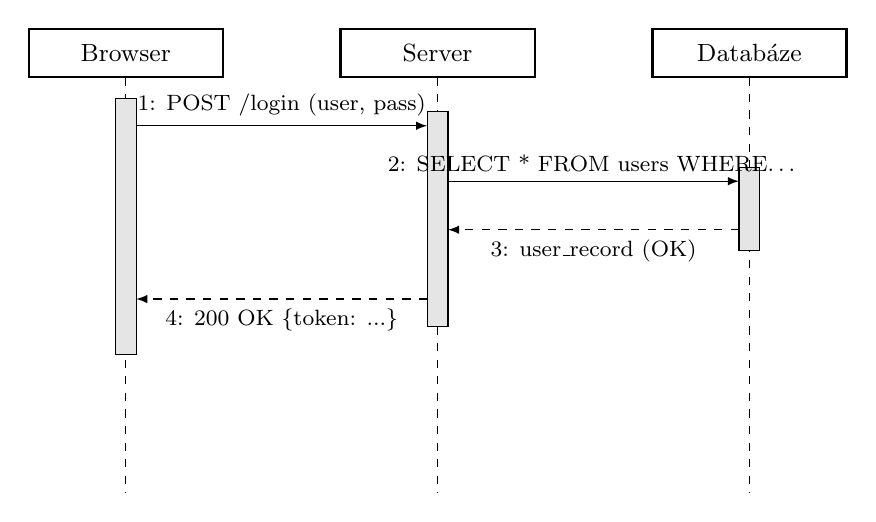
\begin{tikzpicture}[font=\small, scale=0.88, >=latex]
  % Participants (boxes)
  \draw[thick] (0,5.5) rectangle (2.8,6.2);
  \node at (1.4,5.85) {Browser};
  \draw[thick] (4.5,5.5) rectangle (7.3,6.2);
  \node at (5.9,5.85) {Server};
  \draw[thick] (9.0,5.5) rectangle (11.8,6.2);
  \node at (10.4,5.85) {Databáze};
  % Lifelines (dashed vertical)
  \draw[dashed] (1.4,5.5) -- (1.4,-0.5);
  \draw[dashed] (5.9,5.5) -- (5.9,-0.5);
  \draw[dashed] (10.4,5.5) -- (10.4,-0.5);
  % Activation boxes
  \draw[fill=gray!20] (1.25,1.5) rectangle (1.55,5.2);   % Browser active
  \draw[fill=gray!20] (5.75,1.9) rectangle (6.05,5.0);   % Server active
  \draw[fill=gray!20] (10.25,3.0) rectangle (10.55,4.2); % DB active
  % Messages
  \draw[->] (1.55,4.8) -- (5.75,4.8)
    node[midway,above,font=\footnotesize] {1: POST /login (user, pass)};
  \draw[->] (6.05,4.0) -- (10.25,4.0)
    node[midway,above,font=\footnotesize] {2: SELECT * FROM users WHERE\ldots};
  \draw[dashed,->] (10.25,3.3) -- (6.05,3.3)
    node[midway,below,font=\footnotesize] {3: user\_record (OK)};
  \draw[dashed,->] (5.75,2.3) -- (1.55,2.3)
    node[midway,below,font=\footnotesize] {4: 200 OK \{token: ...\}};
\end{tikzpicture}
\caption{Ukázka sekvenčního diagramu -- přihlášení uživatele}
\label{fig:seqdiag}
\end{figure}

\subsubsection{Diagram aktivit (Activity Diagram)}

Zobrazuje tok řízení a dat v procesu nebo algoritmu. Podobný vývojovému diagramu.

\textbf{Elementy:}
\begin{itemize}
  \item \textbf{Počáteční uzel} -- plný kruh
  \item \textbf{Aktivita (Action)} -- zaoblený obdélník
  \item \textbf{Rozhodovací uzel (Decision)} -- diamant; podmíněné větvení
  \item \textbf{Fork/Join} -- tučná vodorovná čára; paralelní větve
  \item \textbf{Swimlanes (plavecké dráhy)} -- oddělení aktivit podle role/zodpovědnosti
  \item \textbf{Koncový uzel} -- plný kruh s kroužkem
\end{itemize}

\begin{figure}[H]
\centering
\begin{tikzpicture}[
  font=\small, >=latex,
  act/.style={rectangle, draw, rounded corners=4pt,
              minimum width=3.8cm, minimum height=0.65cm, align=center},
  dec/.style={diamond, draw, shape aspect=2.5,
              minimum width=3.8cm, minimum height=0.65cm, align=center, font=\footnotesize}
]
  % Start node
  \node[circle, fill=black, minimum size=9pt, inner sep=0pt] (start) at (0,9.2) {};
  % Activities
  \node[act] (pick)  at (0,8.0) {Vybrat produkt};
  \node[dec] (stock) at (0,6.6) {Na skladě?};
  \node[act] (cart)  at (0,5.0) {Přidat do košíku};
  \node[act] (pay)   at (0,3.5) {Zaplatit};
  \node[act] (alt)   at (4.5,6.6) {Zobrazit alternativy};
  % End node
  \node[circle, draw, thick, minimum size=14pt, inner sep=0pt] (endring) at (0,2.0) {};
  \node[circle, fill=black, minimum size=8pt, inner sep=0pt] at (0,2.0) {};
  % Arrows
  \draw[->] (start) -- (pick);
  \draw[->] (pick) -- (stock);
  \draw[->] (stock) -- node[right,font=\footnotesize] {Ano} (cart);
  \draw[->] (cart) -- (pay);
  \draw[->] (pay) -- (endring);
  \draw[->] (stock) -- node[above,font=\footnotesize] {Ne} (alt);
  % Loop back from alt to pick (bent path)
  \draw[->] (alt.north) -- ++(0,0.6) -| (pick.east);
\end{tikzpicture}
\caption{Ukázka diagramu aktivit -- proces objednávky}
\label{fig:actdiag}
\end{figure}

%=============================================================================
\subsection{Návrhové vzory (GoF Design Patterns)}
%=============================================================================

\textbf{Návrhové vzory} jsou opakovaně použitelná řešení často se vyskytujících problémů při návrhu softwaru.
Katalog 23 vzorů (Gang of Four, 1994) je rozdělen do tří skupin.

\subsubsection{Tvořivé vzory (Creational Patterns)}

\paragraph{Singleton}
Zajistí, že třída má pouze jednu instanci, a poskytne globální přístupový bod.
\begin{lstlisting}[language=Java, caption=Singleton]
public class Konfigurace {
    private static Konfigurace instance;

    private Konfigurace() { }

    public static synchronized Konfigurace getInstance() {
        if (instance == null) instance = new Konfigurace();
        return instance;
    }
}
\end{lstlisting}

\paragraph{Factory Method}
Definuje rozhraní pro vytváření objektů, ale nechá podtřídy rozhodnout, které třídy instancovat.
Odstraní závislost kódu na konkrétních třídách.

\paragraph{Abstract Factory}
Poskytuje rozhraní pro vytváření rodin příbuzných objektů bez specifikace jejich konkrétních tříd.
Příklad: GUI toolkity (WindowsButton, MacButton implementují abstraktní Button).

\paragraph{Builder}
Odděluje konstrukci komplexního objektu od jeho reprezentace.
Vhodné pro objekty s mnoha volitelných parametrů.

\paragraph{Prototype}
Vytváří nové objekty klonováním existujícího.

\subsubsection{Strukturální vzory (Structural Patterns)}

\paragraph{Adapter}
Umožní spolupráci tříd s nekompatibilními rozhraními. Obalí existující třídu novým rozhraním.
Příklad: adaptér mezi evropskou a americkou zástrčkou.

\paragraph{Facade}
Poskytne zjednodušené rozhraní ke složitému subsystému.
Příklad: třída \texttt{Computer} s metodou \texttt{start()}, která skryje inicializaci CPU, RAM, HDD.

\paragraph{Decorator}
Dynamicky přidá objektu nové chování bez modifikace jeho třídy. Obalí objekt dekorátorem.
Příklad: \texttt{BufferedReader} obalí \texttt{FileReader} a přidá bufferování.

\paragraph{Composite}
Složí objekty do stromové struktury; klienti s nimi pracují uniformně (jedna metoda pro list i uzel).

\paragraph{Proxy}
Zastupuje jiný objekt; řídí přístup k němu. Typy: vzdálený proxy, virtuální proxy, ochranný proxy.

\subsubsection{Vzory chování (Behavioral Patterns)}

\paragraph{Observer (Pozorovatel)}
Definuje závislost 1:N; při změně stavu se notifikují všichni závislí pozorovatelé.
Příklad: EventListener v GUI, MVC architektura (Model notifikuje View).

\begin{lstlisting}[language=Java, caption=Observer]
interface Pozorovatel {
    void update(String zprava);
}
class PredmetPozorovani {
    private List<Pozorovatel> pozorovatele = new ArrayList<>();
    public void pridat(Pozorovatel p) { pozorovatele.add(p); }
    public void notifikovat(String z) {
        pozorovatele.forEach(p -> p.update(z));
    }
}
\end{lstlisting}

\paragraph{Strategy (Strategie)}
Definuje rodinu algoritmů, zapouzdří je a umožní jejich záměnu.
Příklad: různé způsoby řazení (BubbleSort, QuickSort) implementující rozhraní \texttt{SortStrategy}.

\paragraph{Command (Příkaz)}
Zapouzdří požadavek jako objekt; podporuje undo/redo, logování, fronta příkazů.

\paragraph{Template Method}
Definuje kostru algoritmu v základní třídě a nechá podtřídy doplnit konkrétní kroky.

\paragraph{Iterator}
Poskytne sekvenční přístup k prvkům kolekce bez odhalení její interní struktury.

%=============================================================================
\subsection{Metodiky vývoje IS}
%=============================================================================

\subsubsection{Tradiční (rigorózní) metodiky}

\paragraph{Vodopádový model (Waterfall)}
Sekvenční fáze: analýza $\to$ návrh $\to$ implementace $\to$ testování $\to$ nasazení.
\begin{itemize}
  \item \textbf{Výhody:} jasné fáze, snadná správa, dokumentace
  \item \textbf{Nevýhody:} rigidní, obtížné reagovat na změny požadavků, testování až na konci
\end{itemize}

\paragraph{RUP (Rational Unified Process)}
Iterativní rámec; 4 fáze (Inception, Elaboration, Construction, Transition) s opakujícími se iteracemi.

\subsubsection{Agilní metodiky}

\textbf{Agile Manifesto (2001)} -- 4 hodnoty a 12 principů agilního vývoje.
Hodnoty: individuality nad procesy, funkční SW nad dokumentací, spolupráce se zákazníkem nad smlouvou, reagování na změny nad dodržováním plánu.

\paragraph{Scrum}
Nejrozšířenější agilní rámec.
\begin{itemize}
  \item \textbf{Role:} Product Owner (PO), Scrum Master (SM), Development Team (3--9 lidí)
  \item \textbf{Artefakty:} Product Backlog (seznam požadavků), Sprint Backlog, Increment (fungující SW)
  \item \textbf{Events:} Sprint (1--4 týdny), Sprint Planning, Daily Scrum (15 min), Sprint Review, Sprint Retrospective
  \item Burndown chart sleduje zbývající práci ve Sprintu
\end{itemize}

\paragraph{Crystal}
Rodina metodik (Crystal Clear, Yellow, Orange, Red) přizpůsobená velikosti a kritičnosti projektu.
\begin{itemize}
  \item Crystal Clear: 6--8 lidí, nekritické systémy
  \item Principy: přímá komunikace, reflexe, osmotická komunikace
\end{itemize}

\paragraph{DSDM (Dynamic Systems Development Method)}
Iterativní a inkrementální metodika; fixuje čas a náklady, variabilní je rozsah (MoSCoW prioritizace).
\begin{itemize}
  \item \textbf{MoSCoW:} Must have, Should have, Could have, Won't have
  \item Fáze: Pre-project, Feasibility, Foundation, Exploration, Engineering, Deployment
\end{itemize}

\paragraph{ASD (Adaptive Software Development)}
\begin{itemize}
  \item Cyklus: Speculate (plánování) $\to$ Collaborate (vývoj) $\to$ Learn (hodnocení)
  \item Zaměřen na vysoce turbulentní prostředí
\end{itemize}

\paragraph{Lean Software Development}
Přenesení principů Lean manufacturingu do SW vývoje (Toyota Production System):
\begin{itemize}
  \item 7 principů: eliminuj plýtvání, zesiluj učení, rozhoduj pozdě, dodávej rychle, zmocni tým, buduj integritu, viditelnost celku
\end{itemize}

\paragraph{FDD (Feature Driven Development)}
\begin{itemize}
  \item Vývoj řízený funkcemi (features); iterace 2 týdny
  \item 5 aktivit: Develop Overall Model, Build Feature List, Plan by Feature, Design by Feature, Build by Feature
\end{itemize}

\paragraph{XP (Extreme Programming)}
Agilní metodika s důrazem na technické praktiky:
\begin{itemize}
  \item \textbf{Párové programování} -- dva vývojáři u jednoho počítače; průběžná revize kódu
  \item \textbf{TDD} -- testy před implementací
  \item \textbf{Kontinuální integrace} -- časté buildy a testy
  \item \textbf{Refaktoring} -- průběžné zlepšování struktury kódu
  \item \textbf{Jednoduché návrhy} -- YAGNI (You Aren't Gonna Need It)
  \item \textbf{Kolektivní vlastnictví kódu} -- každý může měnit jakýkoli kód
  \item Krátké iterace (1--2 týdny), zákazník je přímo v týmu
\end{itemize}

\subsubsection{Srovnání přístupů}

\begin{center}
\begin{tabular}{lll}
\toprule
\textbf{Vlastnost} & \textbf{Agilní} & \textbf{Tradiční (Waterfall)} \\
\midrule
Požadavky & Proměnné, iterativní & Fixní, předem definované \\
Dokumentace & Minimální, funkční SW & Rozsáhlá \\
Zákazník & Průběžně zapojen & Zapojen na začátku a konci \\
Dodávka & Inkrementální & Jednorázová \\
Tým & Malý, self-organizing & Hierarchický \\
Vhodné pro & Nejasné požadavky & Stabilní, dobře definované projekty \\
\bottomrule
\end{tabular}
\end{center}

%=============================================================================
\subsection{Architektonické vzory a CMMI}
%=============================================================================

\subsubsection{Architektonické vzory}

Architektonické vzory popisují strukturu celého systému na vysoké úrovni:

\begin{itemize}
  \item \textbf{Vrstvená architektura (Layers)} -- systém rozdělen do horizontálních vrstev;
    každá vrstva poskytuje služby vrstvě nad ní (UI $\to$ Business Logic $\to$ Data Access $\to$ DB);
    výhoda: oddělení zodpovědností, snadná výměna vrstvy
  \item \textbf{Pipes and Filters} -- data procházejí sekvencí filtrů (transformací) propojených rourami;
    příklady: Unix pipeline, ETL procesy, kompilátory
  \item \textbf{Shared Repository (Blackboard)} -- komponenty sdílejí společné datové úložiště;
    vhodné pro komplexní problémy řešené více spolupracujícími komponentami; příklad: IDE (editor, compiler, debugger)
  \item \textbf{MVC (Model-View-Controller)} -- oddělení dat (Model), prezentace (View) a logiky (Controller);
    Model notifikuje View o změnách (Observer pattern); příklady: Spring MVC, Ruby on Rails, ASP.NET MVC
  \item \textbf{Klient-Server} -- server poskytuje zdroje/služby; klient o ně žádá; příklady: web (HTTP), e-mail (SMTP)
  \item \textbf{Peer-to-Peer (P2P)} -- každý uzel je současně klient i server; příklady: BitTorrent, blockchain
  \item \textbf{Event-driven} -- komponenty komunikují přes události (events); volná vazba;
    příklady: GUI aplikace, microservices s message brokery (Kafka, RabbitMQ)
\end{itemize}

\subsubsection{CMMI (Capability Maturity Model Integration)}

\textbf{CMMI} je rámec pro hodnocení a zlepšování procesní zralosti organizací vyvíjejících software.
Definuje 5 úrovní zralosti:

\begin{enumerate}
  \item \textbf{Initial (Počáteční)} -- procesy chaotické, ad-hoc; úspěch závisí na individuu
  \item \textbf{Managed (Řízený)} -- projekty jsou plánované a sledované; základní projektové procesy
  \item \textbf{Defined (Definovaný)} -- procesy standardizované na úrovni organizace; popsány v procesním modelu
  \item \textbf{Quantitatively Managed (Kvantitativně řízený)} -- procesy měřeny a statisticky řízeny; předvídatelnost
  \item \textbf{Optimizing (Optimalizující)} -- kontinuální zlepšování procesů; inovace; prevence defektů
\end{enumerate}

%=============================================================================
\subsection{Software Quality Assurance (SQA)}
%=============================================================================

\subsubsection{Co je SQA a proč na ní záleží}

\textbf{Software Quality Assurance (SQA)} je systematický soubor činností, jejichž cílem je zajistit, že softwarový produkt splňuje definované požadavky na kvalitu a je dodáván bez kritických chyb.

\paragraph{SQA vs. QC -- důležité rozlišení}
\begin{itemize}
  \item \textbf{QA (Quality Assurance)} -- \textit{preventivní}; zaměřuje se na \textbf{procesy} vývoje;
    cílem je zabránit vzniku defektů (správné code review, správná metodika, testovací strategie)
  \item \textbf{QC (Quality Control)} -- \textit{detektivní}; zaměřuje se na \textbf{produkt};
    hledá defekty které již vznikly (testování, inspekce výstupů)
\end{itemize}

\textbf{Proč SQA záleží v praxi:}
\begin{itemize}
  \item Chyba nalezená při \textbf{code review} stojí hodiny práce
  \item Chyba nalezená při \textbf{testování} stojí dny práce (oprava + regrese)
  \item Chyba nalezená \textbf{zákazníkem v produkci} stojí týdny + poškozená reputace
  \item Příklad: Boeing 737 MAX -- chyba MCAS softwaru; NASA Mars Climate Orbiter -- chyba jednotek (imperial vs. metric)
\end{itemize}

\subsubsection{Dimenze kvality softwaru -- ISO/IEC 25010}

\textbf{ISO/IEC 25010} (SQuaRE) definuje 8 charakteristik kvality produktu s konkrétními příklady z praxe:

\begin{itemize}
  \item \textbf{Funkčnost} -- dělá systém to, co má?
    \newline\textit{Příklad: platební brána správně odečte částku z účtu a zašle potvrzení}
  \item \textbf{Výkonnostní efektivita} -- jak rychle a s jakými zdroji?
    \newline\textit{Příklad: stránka e-shopu se načte do 2 s i při 10\,000 souběžných uživatelích}
  \item \textbf{Spolehlivost} -- funguje systém správně i za nepříznivých podmínek?
    \newline\textit{Příklad: bankovní systém dosahuje 99{,}99\,\% dostupnosti (méně než 1 hod výpadku/rok)}
  \item \textbf{Použitelnost} -- mohou uživatelé systém efektivně používat?
    \newline\textit{Příklad: nový zaměstnanec zvládne základní operace v CRM bez školení do 30 minut}
  \item \textbf{Bezpečnost} -- jsou data a funkce chráněny před neoprávněným přístupem?
    \newline\textit{Příklad: hesla jsou ukládána jako bcrypt hash, ne plaintext; HTTPS everywhere}
  \item \textbf{Udržovatelnost} -- lze systém snadno měnit a rozšiřovat?
    \newline\textit{Příklad: přidání nové platební metody nevyžaduje změny ve více než 3 souborech}
  \item \textbf{Přenositelnost} -- lze systém nasadit v různých prostředích?
    \newline\textit{Příklad: aplikace běží na Windows, Linux i macOS; Docker kontejner nasaditelný na AWS/Azure}
  \item \textbf{Kompatibilita} -- funguje systém správně vedle jiných systémů?
    \newline\textit{Příklad: REST API vrací data ve formátu kompatibilním s mobilní i webovou aplikací}
\end{itemize}

\subsubsection{Procesy SQA -- s příklady z praxe}

\paragraph{1. Revize kódu (Code Review)}
Inspektor (kolega nebo nástroj) prochází kód před mergem do hlavní větve.

\textbf{Jak probíhá v praxi (GitHub/GitLab Pull Request flow):}
\begin{enumerate}
  \item Vývojář vytvoří feature branch a napíše kód
  \item Otevře Pull Request (PR) -- popis změny, jaké testy přidal
  \item 1--2 kolegové zkontrolují: logika, bezpečnostní díry, dodržení konvencí, duplicity
  \item Reviewer buď approves nebo přidá komentáře s požadovanými změnami
  \item Po schválení se branch merguje do \texttt{main}
\end{enumerate}

\textbf{Co code review zachytí:}
překlepy v podmínkách (\texttt{=} místo \texttt{==}), SQL injection, chybějící null check, porušení SOLID,
zbytečná složitost, chybějící testy.

\paragraph{2. Statická analýza kódu}
Automatizované nástroje analyzují zdrojový kód \textbf{bez jeho spuštění}:

\begin{itemize}
  \item \textbf{SonarQube} -- identifikuje bugs, code smells, bezpečnostní zranitelnosti, technický dluh;
    integruje se do CI/CD pipeline; přiřazuje rating A--E
  \item \textbf{Checkstyle / PMD / SpotBugs} -- Java; kontrola coding conventions, potenciální chyby
  \item \textbf{ESLint / TSLint} -- JavaScript/TypeScript; syntax, konvence, potenciální chyby
\end{itemize}

\textit{Příklad: SonarQube v CI pipeline odmítne merge pokud code coverage klesne pod 80\,\% nebo přibyde kritická zranitelnost.}

\paragraph{3. Testování -- testovací pyramida}

\begin{center}
\begin{tabular}{llll}
\toprule
\textbf{Typ testu} & \textbf{Co testuje} & \textbf{Rychlost} & \textbf{Příklad} \\
\midrule
\textbf{Unit testy} & Izolovaná třída/metoda & Sekundy & \texttt{kalkulacka.secti(2,3) == 5} \\
\textbf{Integrační} & Spolupráce komponent & Minuty & Service + databáze vrátí správný záznam \\
\textbf{Systémové} & Celý systém end-to-end & Minuty & Uživatel se přihlásí a vidí svůj profil \\
\textbf{UAT} & Akceptace zákazníkem & Hodiny & Zákazník potvrdí, že objednávka funguje \\
\textbf{Zátěžové} & Výkon pod zátěží & Hodiny & 1000 users/s, response time $<$ 500 ms \\
\bottomrule
\end{tabular}
\end{center}

\textbf{Testovací pyramida:} základna = mnoho unit testů (levné, rychlé); střed = integrační testy;
vrchol = málo E2E testů (drahé, pomalé). Čím výše v pyramidě, tím dražší oprava chyby.

\paragraph{4. CI/CD -- Continuous Integration / Continuous Deployment}
Každý commit spustí automatický řetěz kontrol:

\begin{center}
\begin{tabular}{lll}
\toprule
\textbf{Krok} & \textbf{Nástroj} & \textbf{Co dělá} \\
\midrule
Checkout kódu & GitHub Actions / GitLab CI & Stáhne větev \\
Build & Maven, Gradle, npm & Zkompiluje projekt \\
Unit testy & JUnit, pytest & Spustí testy, musí 100\,\% projít \\
Statická analýza & SonarQube & Kontrola kvality kódu \\
Integrační testy & Testcontainers, DB v Dockeru & Testy s reálnou DB \\
Security scan & OWASP Dependency-Check & Zranitelné závislosti? \\
Deploy (staging) & Kubernetes, Helm & Nasazení na testovací prostředí \\
E2E testy & Selenium, Cypress & Testy UI v prohlížeči \\
Deploy (produkce) & -- & Pouze pokud vše prošlo \\
\bottomrule
\end{tabular}
\end{center}

\textit{Příklad: tým v Spotify provede přes 1000 deployů denně -- to je možné jen s plně automatizovaným CI/CD.}

\paragraph{5. Metriky kvality kódu}
\begin{itemize}
  \item \textbf{Code coverage} -- \% kódu pokrytého testy; cíl typicky $\geq$80\,\%;
    \textit{pozor: 100\,\% coverage neznamená 0 bugů -- záleží na kvalitě assertů}
  \item \textbf{Technický dluh (Technical Debt)} -- množství práce potřebné k uvedení kódu do ideálního stavu;
    měří ho SonarQube v hodinách/dnech
  \item \textbf{Cyklomatická složitost} -- počet nezávislých cest kódem; hodnota $>$10 signalizuje
    příliš složitou metodu, která by se měla rozdělit
  \item \textbf{MTTR (Mean Time to Repair)} -- průměrná doba od detekce incidentu po jeho vyřešení;
    klíčová metrika DevOps týmů
  \item \textbf{Defect density} -- počet bugů na 1000 řádků kódu (KLOC); benchmark: $<$1 bug/KLOC
\end{itemize}

\begin{profesorbox}[Otázky profesorů k tématu: Softwarové inženýrství]
\textbf{Vojíř Stanislav, Ing., Ph.D.}
\begin{itemize}
  \item Popište návrhový vzor Observer a jeho použití.
  \item Jak funguje Scrum? Jaké jsou jeho artefakty a role?
  \item Jaký je rozdíl mezi agilním a vodopádovým modelem?
\end{itemize}
\textbf{Chudán David, Ing., Ph.D.}
\begin{itemize}
  \item Jaké UML diagramy znáte? Který byste použil pro popis interakce mezi objekty?
  \item Co je návrhový vzor a proč jsou důležité?
\end{itemize}
\textbf{Komise: Svátek, Chlapek, Zbořil}
\begin{itemize}
  \item Jaké jsou základní principy agilního vývoje?
  \item Popište diagram případů užití a jeho elementy.
\end{itemize}
\textbf{Sládek Pavel, Ing., Ph.D.}
\begin{itemize}
  \item Co je TDD a jak se liší od tradičního testování?
  \item Jaký je rozdíl mezi Singleton a Factory Method?
\end{itemize}
\textbf{Pour Jan, doc. Ing., CSc.}
\begin{itemize}
  \item Jaké jsou fáze metodiky DSDM?
  \item Co je SQA a jaké procesy zahrnuje?
\end{itemize}
\end{profesorbox}
